\documentclass[cn]{homework}

\title{作业11}

\begin{document}
    \maketitle
    \problem
    % TODO Mindmap

    \problem
    \subsection{INDPROD}
    先画出时序图与PACF(\cref{fig:INDPROD}),
    很明显可以判断出是非平稳的,同时由PACF可以推测,拟合ADF
    的AR模型的截断阶数在1,2左右。
    
    \begin{figure}[h]
        \centering
        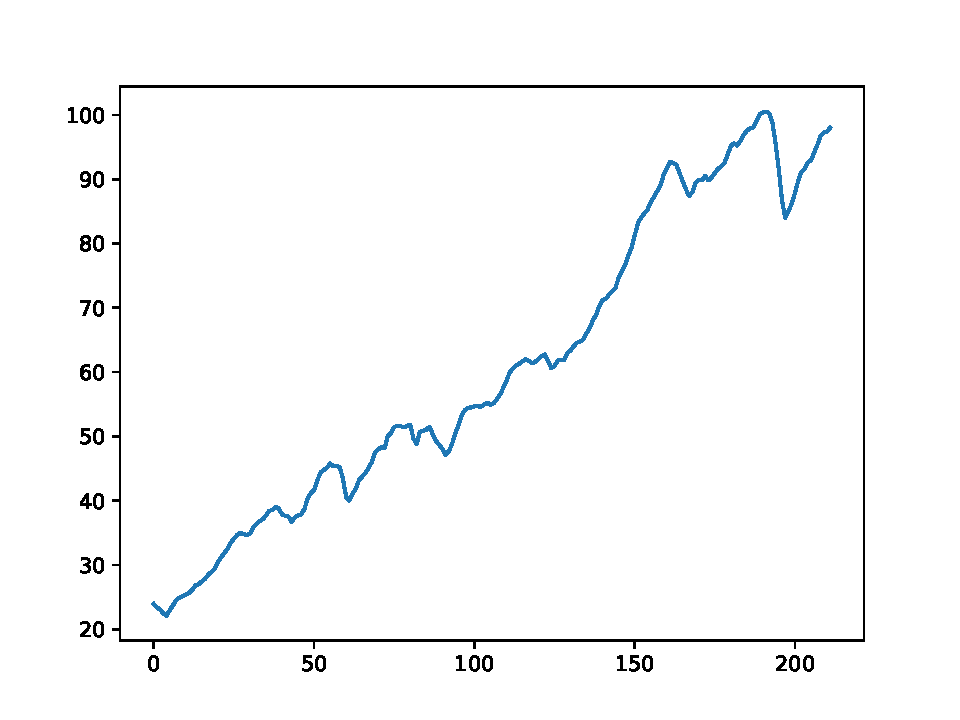
\includegraphics[width=0.48\textwidth]{INDPROD-trend}
        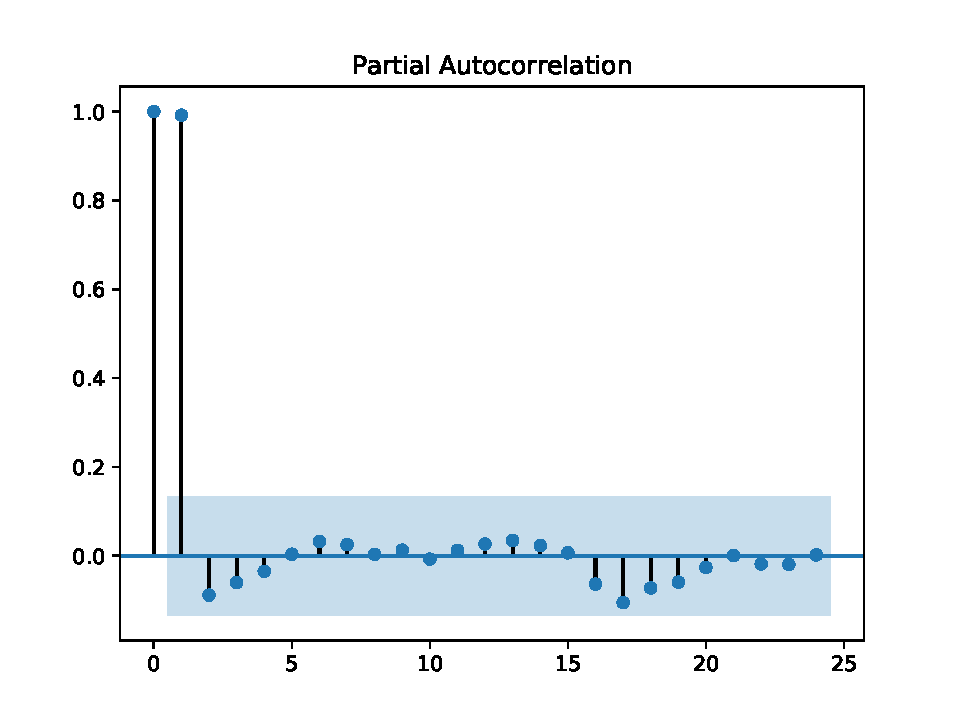
\includegraphics[width=0.48\textwidth]{INDPROD-pacf}
        \caption{INDPROD}
        \label{fig:INDPROD}
    \end{figure}

    先用AR($p$)尝试拟合模型以选择一个最佳的数据生成模型。
    从$p=12$开始依次拟合,得到不同滞后阶数的AIC与BIC
    如\cref{tab: INDPROD ABIC},从而知以AIC为准$p=3$最佳,
    BIC以$p=2$最佳,但$p=2$与$p=3$的AIC差距不如BIC差距,
    以及$p=2$阶数更低,故我们有理由选择AR(2)作为数据生成模型。

    \begin{margintable}
        \centering
        \begin{tabular}{ccc}
            \toprule
            $p$ & AIC & BIC \\
            \midrule
            12 & -0.664 & -0.45 \\
            11 & -0.662 & -0.465 \\
            10 & -0.677 & -0.497 \\
            9 & -0.681 & -0.518 \\
            8 & -0.694 & -0.547 \\
            7 & -0.698 & -0.569 \\
            6 & -0.707 & -0.594 \\
            5 & -0.709 & -0.613 \\
            4 & -0.695 & -0.615 \\
            3 & -0.708 & -0.644 \\
            2 & -0.697 & -0.649 \\
            1 & -0.088 & -0.056 \\
            \bottomrule
        \end{tabular}
        \caption{AIC \& BIC}
        \label{tab: INDPROD ABIC}
    \end{margintable}

    于是做ADF检验可以得到$t=-0.653$以及相应p值为0.859,
    显著大于0.05,从而无法拒绝具有单位根的原假设。

    选取推荐的残差自相关最大阶数$q=3$做pp检验可知,
    修正$rho$统计量$Z_\rho=-0.390$,修正$\tau$统计量
    $Z_\tau=-0.425$,相应p值分别为0.934,0.906,都显著高于0.05,
    从而无法拒绝具有单位根的原假设。

    \subsection{rGDP}
    先对数据进行对数变换,画出时序图与PACF如\cref{fig:rGDP},
    也能很明显地看出数据是非平稳的,同时截断阶数差不多在2,3左右。
    \begin{figure}[h]
        \centering
        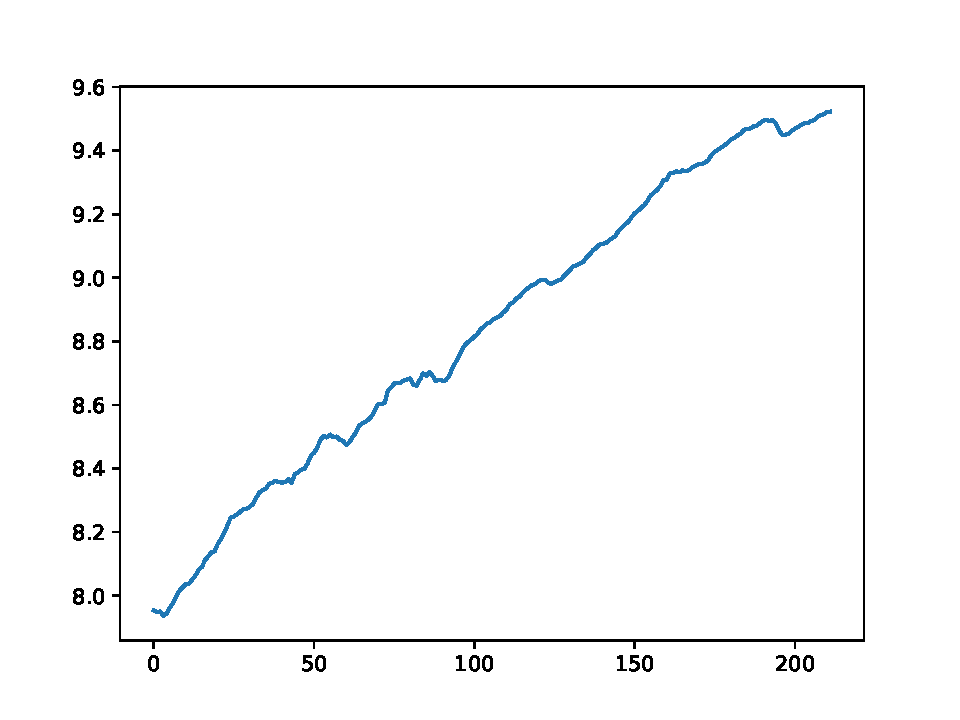
\includegraphics[width=0.48\textwidth]{rGDP-trend}
        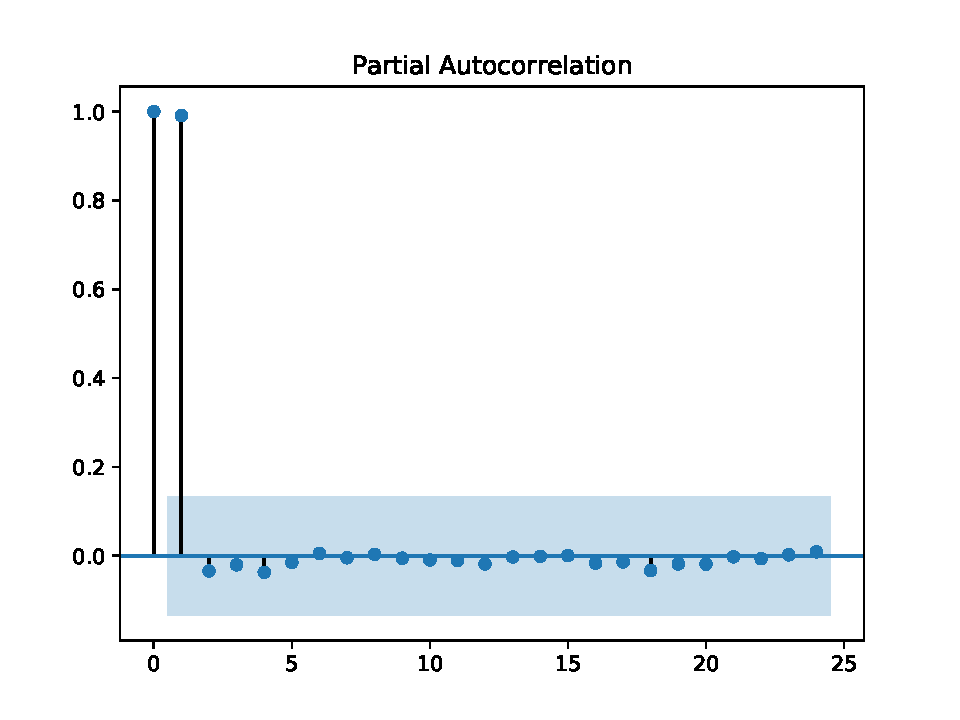
\includegraphics[width=0.48\textwidth]{rGDP-pacf}
        \caption{rGDP}
        \label{fig:rGDP}
    \end{figure}

    从$p=12$开始不断减少尝试拟合AR($p$),得到AIC与BIC如\cref{tab:rGDP ABIC},
    AIC以$p=6$最佳,BIC以$p=3$最佳,于是选择较小的$p=3$做AR模型。
    做ADF检验知$t=-2.648$以及相应的p值$0.083$,显著高于0.05,从而无法拒绝具有单位根的原假设。
    \begin{margintable}
        \centering
        \begin{tabular}{ccc}
            \toprule
            $p$ & AIC & BIC \\
            \midrule
            12 & -9.588 & -9.373 \\
            11 & -9.599 & -9.402 \\
            10 & -9.614 & -9.434 \\
            9 & -9.61 & -9.447 \\
            8 & -9.623 & -9.477 \\
            7 & -9.629 & -9.5 \\
            6 & -9.641 & -9.528 \\
            5 & -9.623 & -9.527 \\
            4 & -9.633 & -9.553 \\
            3 & -9.628 & -9.564 \\
            2 & -9.607 & -9.559 \\
            1 & -9.472 & -9.44 \\
            \bottomrule
        \end{tabular}        
        \caption{AIC \& BIC}
        \label{tab:rGDP ABIC}
    \end{margintable}

    选取$q=3$做pp检验得到$Z_\rho-0.794,Z_\tau=-2.274$,相应有p值
    $0.904,0.180$,均显著高于0.05,从而无法拒绝具有单位根的原假设。
\end{document}